\documentclass{beamer}
\usetheme{metropolis}
\usepackage{graphicx}
\graphicspath{{../../latex/images/}}
\usepackage{boolexpr}
\usepackage{kpfonts}
\usepackage{caption}
\usepackage{wrapfig}
\usepackage{tkz-graph}
\usepackage{tikz}
\usepackage[labelformat=empty]{caption}
\usepackage[official]{eurosym}

\usepackage{minted}

\usepackage{siunitx}

\usepackage[math]{iwona}
\usepackage{scalerel}
\def\lVert{\mid\!\mid}
\def\rVert{\mid\!\mid}

\usepackage[normalem]{ulem}
\usepackage{mathtools}

\usepackage{../../latex/custom}
\usepackage{amsfonts}

\newcommand{\expe}[2]{\la #1, #2 \ra}

\usepackage{framed}

\newcommand\Wider[2][3em]{%
\makebox[\linewidth][c]{%
  \begin{minipage}{\dimexpr\textwidth+#1\relax}
  \raggedright#2
  \end{minipage}%
  }%
}

\newcommand{\aeur}{\alpha_\text{\euro}}
\newcommand{\adol}{\alpha_\$}
\newcommand{\apou}{\alpha_\text{\pounds}}

\title{Extending JuMP and MathOptInterface}
\date{August 7, 2019}
\author{Beno\^it Legat (UCLouvain)}

\makeatletter
\let\@@magyar@captionfix\relax
\makeatother
\begin{document}
  \maketitle

  \begin{frame}
    \tableofcontents
  \end{frame}

\section{Extending MathOptInterface}

  \begin{frame}[fragile]
    \frametitle{MathOptInterface (MOI)}
    \begin{itemize}
      \item \verb|add_variable(model)|, \verb|add_constrained_variable(model, set)|.
      \item \verb|add_constraint(model, func, set)|, e.g. $2x + 3y = 1$ $\to$ (\verb|2*x + 3*y|)-in-\verb|EqualTo(1.0)|.
      \item \verb|set|, \verb|get| attributes, e.g., \verb|ObjectiveFunction|.
      \item \verb|submit| submittables, e.g., \verb|HeuristicSolution|.
    \end{itemize}
    Extensible framework:
    \begin{itemize}
      \item \alert{Generic} on attribute, function and set types. New ones can be defined \alert{independently}.
      \item Solver-\alert{specific} features easily exposed to JuMP/MOI users through \alert{custom} attributes, e.g. solver specific callbacks.
      \item Expose \alert{specialized} problem structure easily through \alert{custom} functions, sets (e.g. Sum-of-Squares variables/constraints).
    \end{itemize}
  \end{frame}

  \begin{frame}{Semidefinite programming}
    \begin{align*}
      \mini_{Q \in \SymK} \quad & \la C, Q \ra & \maxi_{y \in \R^n} \quad & \la b, y \ra\\
      \subtoq & \la A_i, Q \ra = b_i & \subtoq & \sum_i A_i y_i \preceq C\\
        & Q \succeq 0
    \end{align*}
    \textbf{File format}: SDPA

    \textbf{Solvers}: CSDP, SDPA, DSDP, SDPLR, ...

    \textbf{Variables}: $Q$ block diagonal, nonnegative scalar variables ($1 \times 1$ blocks) or SDP matrices.

    \textbf{Constraints}: Affine equations.
  \end{frame}

\begin{frame}{Interval constraint for SDPA}
\Wider[4em]{
  \begin{center}
    \begin{tikzpicture}[xscale=4.5, yscale=2]
      \tikzset{VertexStyle/.style = {}}
      \Vertex[x=1, y=-1, L={$a^\top x + \beta \ge l$}]{G}
      \Vertex[x=2, y=-1, L={$a^\top x + \beta \le u$}]{L}
      \Vertex[x=1, y=-2, L={$A x + b \in \mathbb{R}_+^1$}]{N}
      \Vertex[x=2, y=-2, L={$A x + b \in \mathbb{R}_-^1$}]{P}
      \Vertex[x=1, y=-3, L={$A x + b \in \{0\}^1$}]{Z}
      \Vertex[x=0, y=0, L={$x \le u$}]{VL}
      \Vertex[x=0, y=-1, L={$x \ge l$}]{VG}
      \Vertex[x=0, y=-2, L={$x \in \mathbb{R}_-^1$}]{VP}
      \tikzset{VertexStyle/.style = {
        shape = rectangle,
        draw
      }}
      \Vertex[x=1, y=0, L={$l \le a^\top x + \beta \le u$}]{I}
      \tikzset{VertexStyle/.style = {
        shape = rounded rectangle,
        draw
      }}
      \Vertex[x=2, y=-3, L={$a^\top x = \beta$}]{E}
      \Vertex[x=0, y=-3, L={$x \in \mathbb{R}_+^1$}]{VN}
      \tikzset{EdgeStyle/.style = {->}}
      \Edge[label={flip}](L)(G)
      \Edge[label={flip}](VP)(VN)
      \Edge[label={flip}](VL)(VG)
      \Edge[label={split}](I)(L)
      \Edge[label={split}](I)(G)
      \Edge[label={vectorize}](G)(N)
      \Edge[label={vectorize}](L)(P)
      \Edge[label={scalarize}](Z)(E)
      \Edge[label={slack}](P)(Z)
      \Edge[label={slack}](N)(Z)
      \Edge[label={slack}](N)(VN)
      \Edge[label={slack}](G)(VG)
      \tikzset{EdgeStyle/.style = {->, pos=0.3}}
      \Edge[label={slack}](G)(E)
      \tikzset{EdgeStyle/.style = {->, bend left=22, pos=0.3}}
      \Edge[label={slack}](P)(VP)
      \tikzset{EdgeStyle/.style = {->, bend left=20, pos=0.7}}
      \Edge[label={vectorize}](VL)(VP)
      \tikzset{EdgeStyle/.style = {->, bend left=25, pos=0.8}}
      \Edge[label={slack}](L)(E)
      \tikzset{EdgeStyle/.style = {->, bend right=20, pos=0.3}}
      \Edge[label={vectorize}](VG)(VN)
      \tikzset{EdgeStyle/.style = {->, bend right=25}}
      \tikzset{EdgeStyle/.style = {->, bend right=60, pos=0.2}}
      \Edge[label={slack}](L)(VL)
      \tikzset{EdgeStyle/.style = {->}}
      \Edge[label={flip}](P)(N)
    \end{tikzpicture}
  \end{center}
}
\end{frame}



\begin{frame}
  \frametitle{Bridges directed hypergraph}
  \vspace{-.2cm}
  \begin{block}{Nodes}
    Node for each set $S$ (variable-in-$S$).

    Node for each constraint $F$-in-$S$.

    Node for each objective function $F$.


  \end{block}
  \vspace{-.2cm}
  \begin{block}{Edges}

    For each edge and ingoing node: outgoing nodes are
    \begin{itemize}
        \item variable-in-$S$ created.
        \item constraints $F$-in-$S$ created.
        \item objective $F$ set.
    \end{itemize}
  \end{block}

\end{frame}

\begin{frame}
  \frametitle{Bridges selection}

  \begin{block}{Multiple dispatch ?}
    Can we use multiple dispatch where node types are method signatures ?

    \textbf{No}.
    Several bridge can transform same types.
    Dispatching on more specialized is not accurate.

    Need to guide choice to supported types.
  \end{block}

  \begin{block}{Just in Time (JIT) bridge selection}
    Types $F$ and $S$ are \alert{not limited} to those defined in MOI $\to$
    \alert{infinitely} many nodes.

    Each bridge defined possible \alert{infinitely} many edges.

    Need to be \alert{lazy} and compute bridge selection JIT when
    type first used.
  \end{block}

\end{frame}

\begin{frame}
  \frametitle{Bridge selection algorithm}
  \textbf{Data}: Set of bridges $B$

  \textbf{Invariant}: $d_\mathcal{V}$, $d_\mathcal{C}$, $d_\mathcal{O}$
  are correct when defined.

  Given new type: compute types $T$ where $d$ should be defined with
  Depth First Search (DFS) from the type: $\mathcal{O}(|B|)$.

  Compute $d$ at the types using Bellman-Ford algorithm: $\mathcal{O}(|T| \cdot |B|)$.
\end{frame}

\section{Dualization extension}

\begin{frame}[fragile]
  Extends MOI by creating a new \alert{layer}.

  Problem given to GLPK is the \alert{dual} of problem given to optimizer.
\begin{minted}{Julia}
optimizer = Dualization.DualOptimizer(GLPK.Optimizer())
# or
model = Model(with_optimizer(() ->
    Dualization.DualOptimizer(GLPK.Optimizer())))
\end{minted}
  Primal (resp. dual) results of optimizer are dual (resp. primal) results of GLPK.
\end{frame}

\begin{frame}[fragile]
\begin{minted}{Julia}
struct DualOptimizer{T, OT <: MOI.ModelLike} <:
        MOI.AbstractOptimizer
    dual_problem::DualProblem{T, OT}
end
struct DualProblem{T, OT <: MOI.ModelLike}
    dual_model::OT
    primal_dual_map::PrimalDualMap{T}
end
function MOI.copy_to(dest::DualOptimizer,
                     src::MOI.ModelLike; kws...)
    dualize(src, dest.dual_problem)
    # ...
end
\end{minted}
\end{frame}

\section{Extending JuMP}

\begin{frame}[fragile]
  \frametitle{Extending JuMP macros}
\begin{minted}{Julia}
@constraint(model, [x + 1, x - y] in MOI.Zeros())
\end{minted}
  Implementation:
\begin{minted}{Julia}
function build_constraint(
    _error::Function,
    func::Vector, set::MOI.AbstractVectorSet)
    return VectorConstraint(x, set)
end
function add_constraint(model, c::AbstractConstraint,
                        name)
    index = MOI.add_constraint(backend(model),
        moi_function(c), moi_set(c))
    ... # set name and shape
    return ConstraintRef(model, index, shape(c))
end
\end{minted}
\end{frame}

\begin{frame}[fragile]
  \frametitle{Extending JuMP macros: Custom set}
\begin{minted}{Julia}
@constraint(model, [x + 1, x - y] in SecondOrderCone())
\end{minted}
  Implementation:
\begin{minted}{Julia}
function build_constraint(_error::Function,
                          f::AbstractVector,
                          s::AbstractVectorSet)
    set = moi_set(s, length(f))
    return build_constraint(_error, f, set)
end
function moi_set(::SecondOrderCone, dim::Int)
  return MOI.SecondOrderCone(dim)
end
\end{minted}
\end{frame}

\begin{frame}[fragile]
  \frametitle{Extending JuMP macros: PSD cone}
\begin{minted}{Julia}
using LinearAlgebra # For Symmetric
@constraint(model, Symmetric([x + 1 x - y
                              x - y y]) in PSDCone())
\end{minted}
  Implementation:
\begin{minted}{Julia}
function build_constraint(_error::Function,
                          Q::Symmetric,
                          ::PSDCone)
    n = LinearAlgebra.checksquare(Q)
    func = [Q[i, j] for j in 1:n for i in 1:j]
    set = MOI.PositiveSemidefiniteConeTriangle(n)
    VectorConstraint(func, set,
                     SymmetricMatrixShape(n))
end
\end{minted}
\end{frame}

\begin{frame}[fragile]
  \frametitle{Adding bridges}
\begin{minted}{Julia}
struct BridgeableConstraint{C, B} <: AbstractConstraint
    constraint::C
    bridge_type::B
end

function add_constraint(model::Model,
                        c::BridgeableConstraint,
                        name::String="")
    add_bridge(model, c.bridge_type)
    return add_constraint(model, c.constraint, name)
end
\end{minted}
\end{frame}

\section{Polyhedra extension}

\begin{frame}[fragile]
  \frametitle{Polyhedra example}
  Creating the hypercube from JuMP:
  \begin{minted}{julia}
model = Model()
@variable(model, 0 <= x[1:n] <= 1)

poly = polyhedron(model, CDDLib.Library(:exact))
  \end{minted}
  Polyhedra constraint:
  \begin{minted}{julia}
simplex = intersect(
    HalfSpace([-1, 0], 0), HalfSpace([0, -1], 0),
    HyperPlane([1, 1], 1))
model = Model()
@variable(model, x[1:2])
@constraint(model, A * x in simplex)
  \end{minted}
\end{frame}

\begin{frame}[fragile]
  \frametitle{JuMP model to polyhedron}
  \begin{minted}{julia}
MOI.Utilities.@model(_MOIModel,
    (), (MOI.EqualTo, MOI.LessThan,), (), (),
    (), (MOI.ScalarAffineFunction,), (), ())
mutable struct LPHRep{T} <: HRepresentation{T}
    model::_MOIModel{T}
    # Cached list of indices
    hyperplane_indices::Union{
        Nothing, Vector{MOI.ConstraintIndex{
          MOI.ScalarAffineFunction{T}, MOI.EqualTo{T}}}}
    hyperplane_indices::Union{
        Nothing, Vector{MOI.ConstraintIndex{
          MOI.ScalarAffineFunction{T}, MOI.LessThan{T}}}}
end
  \end{minted}
\end{frame}

\begin{frame}[fragile]
  \frametitle{Polyhedra constraint: Extending MOI}
  \begin{minted}{julia}
struct PolyhedraOptSet{T, RepT <: Rep{T}} <:
    MOI.AbstractVectorSet
    rep::RepT
end
struct PolyhedraToLPBridge{T, F} <:
    MOI.Bridges.AbstractBridge
    hyperplanes::Vector{MOI.ConstraintIndex{
        F, MOI.EqualTo{T}}}
    halfspaces::Vector{MOI.ConstraintIndex{
        F, MOI.LessThan{T}}}
end
  \end{minted}
\end{frame}
\begin{frame}[fragile]
  \frametitle{Polyhedra constraint: Extending JuMP}
  \begin{minted}{julia}
function JuMP.build_constraint(
    error_fun::Function, func, set::Polyhedra.Rep)
    return JuMP.BridgeableConstraint(
        JuMP.build_constraint(
            error_fun, func, PolyhedraOptSet(set)),
        PolyhedraToLPBridge)
end
  \end{minted}
\end{frame}

\section{Sum-of-Squares extension}

  \begin{frame}{Nonnegative quadratic forms into sum of squares}
    \begin{tikzpicture}
      \draw[->, bend left=30] (-1, 1.6) node[left] {$(x_1, x_2, x_3)$} to (-.1, 1.3);
      \draw[->, bend left=30] (-1, 1.6) to (.9, 1.25);
      \draw[->, bend right=30] (2.1, 2) node[right] {\alert{unique}} to (1.55, 1.35);
      \node at (-.2, 1.2) {$p(x)$};
      \node at (.5, 1.2) {$=$};
      \node at (1.3, 1.2) {$x^\Tr Q x$};
      \node at (-2.4, 0) {$x_1^2 + 2x_1x_2 + 5x_2^2 + 4x_2x_3 + x_3^2$};
      \node at (.5, 0) {$=$};
      \node at (2.4, 0) {$x^\Tr \begin{pmatrix}1 & 1 & 0\\1 & 5 & 2\\ 0 & 2 & 1\end{pmatrix} x$};
      \node at (-1, -1.5) {$p(x) \geq 0$ $\forall x$};
      \node at (1.5, -1.5) {$Q \succeq 0$};
      \node at (.5, -1.5) {$\Longleftrightarrow$};
      \draw[->] (2.5, -1) to node[right] {cholesky} (2.5, -2.5);
      \node at (-3, -3.5) {$(x_1 + x_2)^2 + (2x_2 + x_3)^2$};
      \draw[->] (.2, -3.5) to (-.8, -3.5);
      \node at (3, -3.5) {$x^\Tr \begin{pmatrix}1 & 1 & 0\\0 & 2 & 1\end{pmatrix}^\Tr \begin{pmatrix}1 & 1 & 0\\0 & 2 & 1\end{pmatrix} x$};
    \end{tikzpicture}
  \end{frame}

  \begin{frame}{Nonnegative polynomial into sum of squares}
    \begin{tikzpicture}
      \draw[->, bend left=30] (-1, 1.6) node[left] {$(x_1, x_2, x_3)$} to (-.1, 1.3);
      \draw[->, bend left=20] (.6, 1.6) node[above] {$(x_1, x_1x_2, x_2)$} to (.9, 1.35);
      \draw[->, bend right=30] (2.1, 2) node[right] {\alert{\emph{not} unique}} to (1.55, 1.35);
      \node at (-.1, 1.2) {$p(x)$};
      \node at (.5, 1.2) {$=$};
      \node at (1.3, 1.2) {$X^\Tr Q X$};
      \node at (-2.5, 0) {$x_1^2 + 2x_1^2x_2 + 5x_1^2x_2^2 + 4x_1x_2^2 + x_2^2$};
      \node at (.5, 0) {$=$};
      \node at (2.3, 0) {$X^\Tr \begin{pmatrix}1 & 1 & 0\\1 & 5 & 2\\ 0 & 2 & 1\end{pmatrix} X$};
      \node at (-1, -1.5) {$p(x) \geq 0$ $\forall x$};
      \node at (1.5, -1.5) {$Q \succeq 0$};
      \node at (.5, -1.5) {$\Longleftarrow$};
      \draw[->] (2.5, -1) to node[right] {cholesky} (2.5, -2.5);
      \node at (-3, -3.5) {$(x_1 + x_1x_2)^2 + (2x_1x_2 + x_2)^2$};
      \draw[->] (.2, -3.5) to (-.6, -3.5);
      \node at (3, -3.5) {$X^\Tr \begin{pmatrix}1 & 1 & 0\\0 & 2 & 1\end{pmatrix}^\Tr \begin{pmatrix}1 & 1 & 0\\0 & 2 & 1\end{pmatrix} X$};
    \end{tikzpicture}
  \end{frame}

  \begin{frame}{When is nonnegativity equivalent to sum of squares ?}
    Determining whether a polynomial is nonnegative is \alert{NP-hard}.
    \begin{block}{Hilbert 1888}
      Nonnegativity of $p(x)$ of $n$ variables and degree $2d$ is equivalent to sum of squares in the following three cases:
      \begin{itemize}
        \item $n = 1$ : Univariate polynomials
        \item $2d = 2$ : Quadratic polynomials
        \item $n = 2$, $2d = 4$ : Bivariate quartics
      \end{itemize}
    \end{block}
    \begin{columns}
      \begin{column}{0.7\textwidth}
    \begin{block}{Motzkin 1967}
      First \alert{explicit} example:
      \[ x_1^4x_2^2 + x_1^2x_2^4 + 1 - 3x_1^2x_2^2 \geq 0 \quad \forall x \]
      but is \alert{not} a sum of squares.
    \end{block}
      \end{column}
      \begin{column}{0.3\textwidth}
        \centering
        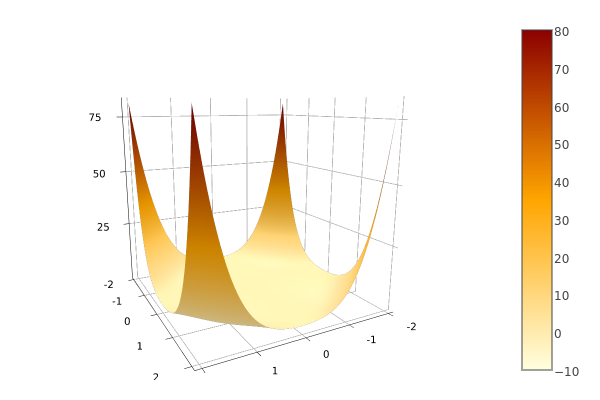
\includegraphics[trim=3cm .7cm 6cm 3cm, clip, width=\textwidth]{motzkin.png}
      \end{column}
    \end{columns}
  \end{frame}

  \begin{frame}
    \frametitle{Theory behind bridges}
    \[ x \in S_1 \Leftrightarrow Ax \in S_2 \qquad AS_1 = S_2 \]
    \[ A^* y \in S_1^* \Leftrightarrow y \in S_2^* \qquad S_1^* = A^* S_2^* \]
    In Lagrangian:
    \[ \langle Ax, y \rangle_2 = \langle x, A^* y \rangle_1 \]
    \vspace{-0.5cm}
    \begin{block}{Transformation of variable-in-$S_2$ to variable-in-$S_1$.}
      \begin{enumerate}
        \item[Primal] Transform value $v$ to $Av$.
        \item[Dual] Transform dual $y$ to $A^{-*}y$.
      \end{enumerate}
    \end{block}
    \begin{block}{Transformation of $f$-in-$S_1$ constraint to $Af$-in-$S_2$ constraint.}

      \begin{enumerate}
        \item[Primal] Transform value $v$ of $Af$ to $A^{-1}v$ of $f$.
        \item[Dual] Transform dual $y$ of $A^*y$.
      \end{enumerate}
    \end{block}
  \end{frame}

\begin{frame}
  \frametitle{Sum-of-Squares bridges}
  Polynomial $p \in \Sigma$ ($p$ is SOS) iff
  $p = X^\Tr Q X$ with $Q \in \mathbb{S}_+$ ($Q$ is PSD).
  Hence $\Sigma = A \mathbb{S}_+$.

  SOSPolnomialBridge: Transformation of variable-in-$\Sigma$ to variable-in-$\mathbb{S}_+$.

  Transformation of contraint $F$-in-$\Sigma$: SlackBridge + SOSPolnomialBridge.
\end{frame}

\begin{frame}
  \frametitle{Result transformations}
  \begin{block}{Constraint Attribute}
    \textbf{Examples}: ConstraintPrimal, ConstraintDual, ConstraintFunction, ConstraintSet, ...

    \alert{Redirected} to bridge when constraint is bridged.
  \end{block}
  New attributes:
  \begin{itemize}
    \item GramMatrixAttribute: Gram matrix $Q$ indexed by $X$.
    \item MomentMatrixAttribute: Moment matrix index by $X$, dual of constraint $Q \in \mathbb{S}_+$.
    \item MomentsAttribute: Vector of moments, dual of constraint $p = X^\top Q X$.
  \end{itemize}
\end{frame}

\begin{frame}[fragile]
  \frametitle{Sum-of-Squares constraint macro}
\begin{minted}{Julia}
@constraint(model, p in SOSCone())
\end{minted}
  Implementation:
\begin{minted}{Julia}
function JuMP.build_constraint(_error::Function, p,
                               cone::SOSCone; kws...)
    coefs = coefficients(p)
    monos = monomials(p)
    set = JuMP.moi_set(cone, monos; kws...)
    shape = PolyJuMP.PolynomialShape(monos)
    return PolyJuMP.bridgeable(
        JuMP.VectorConstraint(coefs, set, shape),
        JuMP.moi_function_type(typeof(coefs)),
        typeof(set)
    )
end
\end{minted}
\end{frame}

\section{Set Programming extension}

\begin{frame}[fragile]
  \frametitle{Example with ellipsoids: Model}
  Maximal volume ellipsoid (determinant):
  \begin{center}
    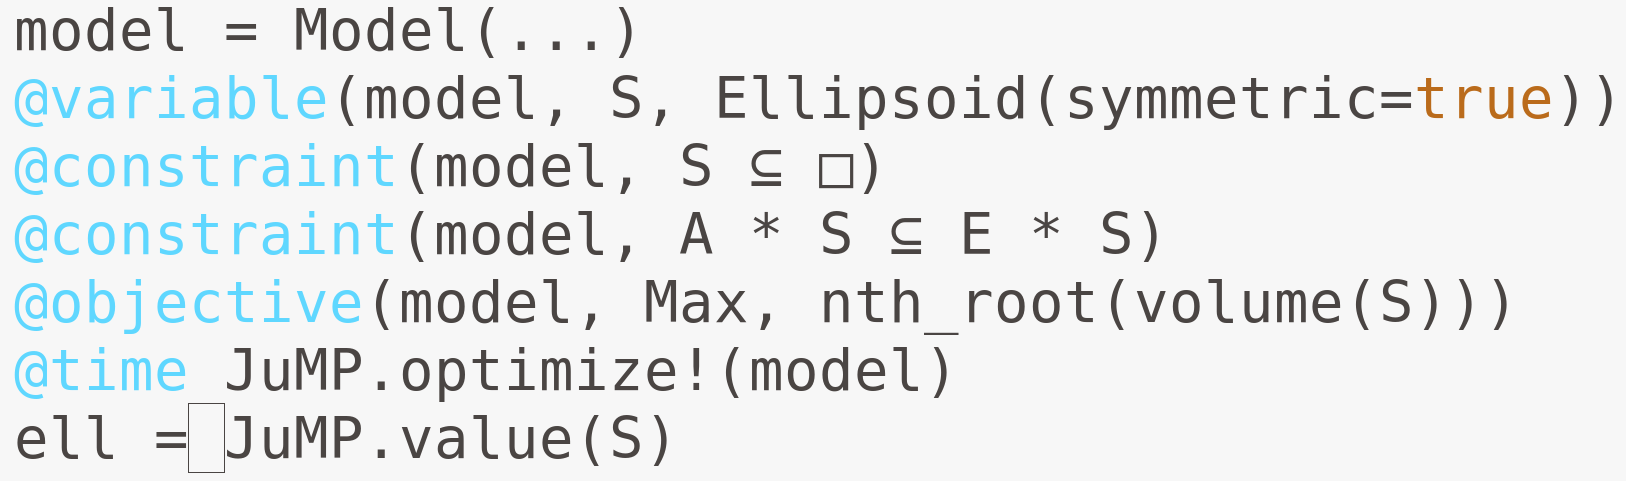
\includegraphics[width=\textwidth]{SetProg_Ellipsoid_AE.png}
  \end{center}
  Maximal sum of the squares of the semi-axes of the ellipsoid (trace):
  \begin{minted}{julia}
@objective(model, Max,
           L1_heuristic(volume(S), [1.0, 1.0]))
  \end{minted}
\end{frame}

\begin{frame}{Example with ellipsoids: Primal Solution}
  \begin{center}
    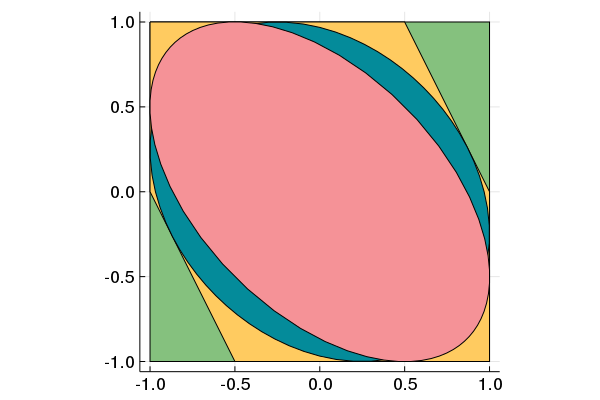
\includegraphics[width=\textwidth]{SimpleControlledInvariantEllipsoid.png}~%
  \end{center}
\end{frame}
\begin{frame}{Example with ellipsoids: Polar Solution}
  \begin{center}
    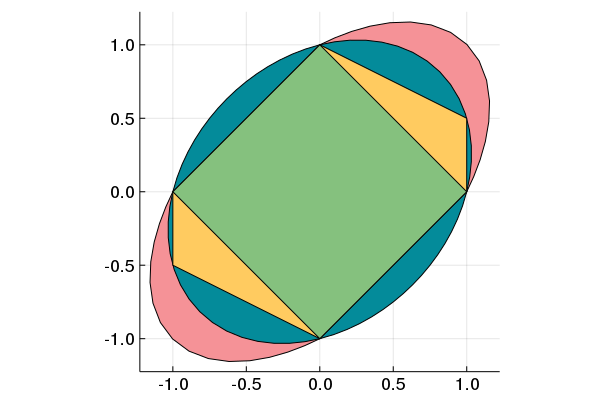
\includegraphics[width=\textwidth]{SimpleControlledInvariantPolarEllipsoid.png}
  \end{center}
\end{frame}

\begin{frame}[fragile]
  \frametitle{Set variables}
  \begin{minted}{julia}
function JuMP.build_variable(
    _error, info::JuMP.VariableInfo,
    set::AbstractSetVariable)
    if info.has_lb || info.has_ub || ...
        _error(...)
    end
    return set
end
function JuMP.add_variable(
    model::JuMP.AbstractModel, set::AbstractSetVariable,
    name::String)
    vref = SetVariableRef(...)
    push!(data(model).variables, vref)
    return vref
end
  \end{minted}
\end{frame}

\begin{frame}
  \frametitle{Parsing set constraints}
  \begin{center}
    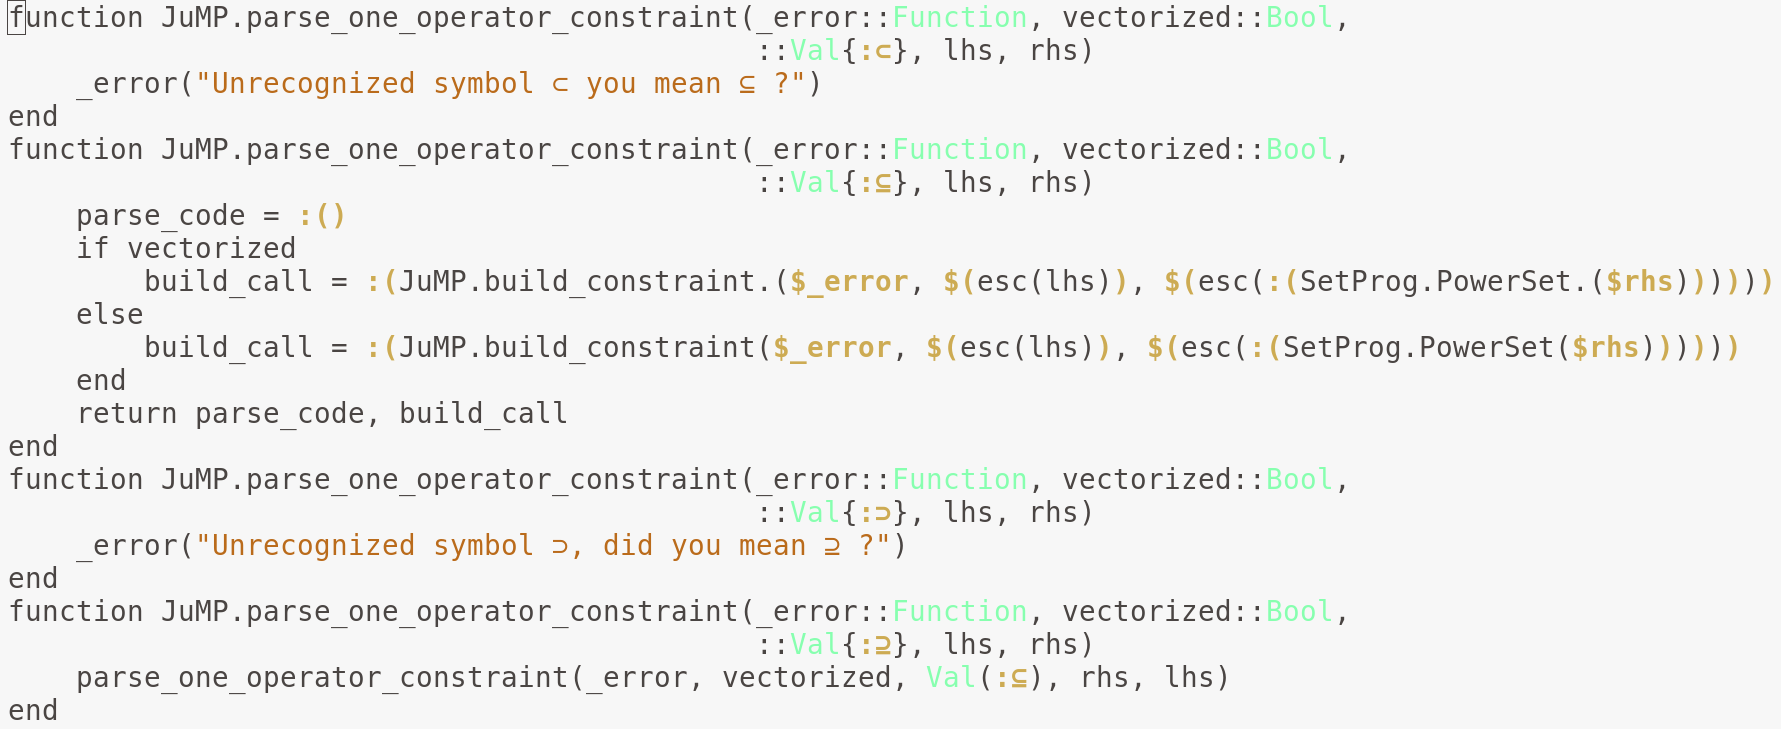
\includegraphics[width=\textwidth]{SetProg_parse_constraint.png}
  \end{center}
\end{frame}

\begin{frame}[fragile]
  \frametitle{Store set constraints}
  \begin{minted}{julia}
function JuMP.build_constraint(
    _error::Function, subset, sup_powerset::PowerSet;
    kws...)
    InclusionConstraint(subset, sup_powerset.set, kws)
end
function JuMP.add_constraint(
    model::JuMP.Model, constraint::SetConstraint,
    name::String="")
    d = data(model)
    index = ConstraintIndex(d.last_index += 1)
    d.constraints[index] = constraint
    d.names[index] = name
    return JuMP.ConstraintRef(model, index, SetShape())
end
  \end{minted}
\end{frame}

\begin{frame}[fragile]
  \frametitle{Optimize hook}
  \verb|create_spaces|: Find dimensions and
  representation (e.g. polar/dual or not)
  \begin{minted}{julia}
function optimize_hook(model::JuMP.AbstractModel; kws...)
    d = data(model)
    clear_spaces(d)
    create_spaces(d)
    load(model, d)
    JuMP.optimize!(model, ignore_optimize_hook = true,
                   kws...)
end
  \end{minted}
\end{frame}

\section{ParameterJuMP extension}

\begin{frame}[fragile]
  \frametitle{ParameterJuMP example}
  \begin{minted}{julia}
model = ModelWithParams(with_optimizer(...))
@variable(model, x)
add_parameter(model, a, 10)
@constraint(model, x >= a)
optimize!(model)
dual(a)

fix(a, 20)
optimize!(model)
  \end{minted}
\end{frame}

\begin{frame}[fragile]
  \frametitle{Adding parametrized constraint}
  \begin{minted}{julia}
function JuMP.build_constraint(
    _error::Function, aff::PAE, set)
    return JuMP.ScalarConstraint(aff, set) # Simplified
end

function JuMP.add_constraint(model::JuMP.Model, c::PAEC,
                             name::String="")
    c_lin = JuMP.ScalarConstraint(c.func.v, c.set)
    cref = JuMP.add_constraint(model, c_lin, name)
    data = model.ext[:params]::ParameterData
    _get_param_dict(data, S)[cref] = c.func.p
    return cref
end
  \end{minted}
\end{frame}

\begin{frame}[fragile]
  \frametitle{Optimize hook}
  \begin{minted}{julia}
function parameter_optimizehook(model::JuMP.Model;
                                kwargs...)
    data = model.ext[:params]::ParameterData

    sync(data)

    ret = JuMP.optimize!(
        model, ignore_optimize_hook = true, kwargs...)

    if !no_duals(data) && JuMP.has_duals(model)
        _update_duals(data)
    end
    return ret
end
  \end{minted}
\end{frame}

\section{StructJuMP extension}

\begin{frame}[fragile]
  \frametitle{Example}
  \begin{minted}{julia}
numScen = 2
m = StructuredModel(num_scenarios=numScen)
@variable(m, x[1:2])
@NLconstraint(m, x[1] + x[2] == 100)
@NLobjective(m, Min, x[1]^2 + x[2]^2 + x[1]*x[2])

for i in 1:numScen
    bl = StructuredModel(parent=m, id=i)
    @variable(bl, y[1:2])
    @NLconstraint(bl, x[1] + y[1] + y[2] >=  0)
    @NLconstraint(bl, x[2] + y[1] + y[2] <= 50)
    @NLobjective(bl, Min, y[1]^2 + y[2]^2 + y[1]*y[2])
end
  \end{minted}
\end{frame}

\begin{frame}[fragile]
  \frametitle{AbstractModel without any MOI backend}
  \begin{minted}{julia}
mutable struct StructuredModel <: JuMP.AbstractModel
    parent::Union{StructuredModel, Nothing}
    # Graph data ...

    nextvaridx::Int
    variables::Dict{Int, JuMP.AbstractVariable}
    varnames::Dict{Int, String}
    nextconidx::Int
    constraints::Dict{Int, JuMP.AbstractConstraint}
    connames::Dict{Int, String}
    objective_sense::MOI.OptimizationSense
    objective_function::JuMP.AbstractJuMPScalar
end
  \end{minted}
\end{frame}

\begin{frame}[fragile]
  \frametitle{Variables}
  \begin{minted}{julia}
struct StructuredVariableRef <: JuMP.AbstractVariableRef
    model::StructuredModel
    idx::Int
end
function JuMP.add_variable(
    model::StructuredModel, v::JuMP.AbstractVariable,
    name::String="")
    model.nextvaridx += 1
    vref = StructuredVariableRef(
        model, model.nextvaridx)
    model.variables[vref.idx] = v
    JuMP.set_name(vref, name)
    return vref
end
  \end{minted}
\end{frame}

\begin{frame}[fragile]
  \frametitle{Constraint}
  \begin{minted}{julia}
struct StructuredConstraintRef
    model::StructuredModel
    idx::Int
end
function JuMP.add_constraint(
    model::StructuredModel, c::JuMP.AbstractConstraint,
    name::String="")
    model.nextconidx += 1
    cref = StructuredConstraintRef(
        model, model.nextconidx)
    model.constraints[cref.idx] = c
    JuMP.set_name(cref, name)
    return cref
end
  \end{minted}
\end{frame}

\begin{frame}[fragile]
  \frametitle{Objective}
  \begin{minted}{julia}
function JuMP.set_objective_sense(
    model::StructuredModel, sense::MOI.OptimizationSense)
    model.objective_sense = sense
end
function JuMP.set_objective_sense(
    model::StructuredModel, f::JuMP.AbstractJuMPScalar)
    model.objective_function = f
end
  \end{minted}
\end{frame}

\begin{frame}[fragile]
  \frametitle{New attribute}
  \begin{minted}{julia}
struct VariableBlock <: MOI.AbstractVariableAttribute
end
  \end{minted}
  \begin{itemize}
    \item Block 0: parent
    \item Block $i$: $i$th children
  \end{itemize}
  \begin{minted}{julia}
optimizer = PIPS.Optimizer()
parent_vars = MOI.add_variables(optimizer, n0)
MOI.set(optimizer, VariableBlock(), parent_vars,
        zeros(n0))
child1_vars = MOI.add_variables(optimizer, n1)
MOI.set(optimizer, VariableBlock(), child_vars,
        zeros(n1))
  \end{minted}
\end{frame}

\section{MomentOpt extension}

\begin{frame}[fragile]
  \frametitle{Example}
  Generalized Moment Problem for
  $$\min_{|x| \le 1, |y| \le 1} x^4y^2 + x^2y^4 -3x^2y^2 + 1$$
  \begin{minted}{julia}
@polyvar x y
f =x^4*y^2 + x^2*y^4 -3x^2*y^2 + 1
K = @set -1 <= x && x <= 1 && -1 <= y && y <= 1
gmp = GMPModel()
@measure(gmp, mu, [x, y], support=K)
@objective(gmp, Min, dot(f, mu))
@constraint(gmp, dot(1, mu) == 1)
relax!(gmp, 2, with_optimizer(CSDP.Optimizer))
  \end{minted}
\end{frame}

\begin{frame}[fragile]
  \frametitle{Model}
  \begin{minted}{julia}
mutable struct GMPModel <: JuMP.AbstractModel
    objective::Union{Nothing, MomObj}
    constraints::Vector{MomCon}
    constraint_names::Vector{String}
    measures::Vector{Measure}

    dual::JuMP.Model
    cref::Dict{Measure, JuMP.ConstraintRef{JuMP.Model}}
    dref::Vector{JuMP.VariableRef}
end
  \end{minted}
\end{frame}

\begin{frame}[fragile]
  \frametitle{Constraint}
  \begin{minted}{julia}
function JuMP.build_constraint(
    _error::Function, aff::AffMomExpr,
    set::MOI.AbstractScalarSet)
    return MomCon(aff, set)
end

function JuMP.add_constraint(
    gmp::GMPModel, momcon::MomCon, name::String="")
    push!(gmp.constraints, momcon)
    push!(gmp.constraint_names, name)
    return ConstraintRef(gmp, length(constraints(gmp)),
                         MomConShape())
end
  \end{minted}
\end{frame}

\begin{frame}[fragile]
  \frametitle{Objective}
  \begin{minted}{julia}
function JuMP.set_objective(
    gmp::GMPModel, sense::MOI.OptimizationSense,
    mom::AbstractMomentExpressionLike)
    gmp.objective = MomObj(sense, mom)
end
  \end{minted}
\end{frame}

\begin{frame}[fragile]
  \frametitle{Relax}
  \begin{minted}{julia}
function relax!(gmp::GMPModel, order::Int,
                optimizer::OptimizerFactory)
    gmp.dual = SOSModel(optimizer)

    # ...

    optimize!(gmp.dual)
end
  \end{minted}
\end{frame}

\begin{frame}[fragile]
  \frametitle{Conclusion}
  Many ways to extend JuMP/MOI:
  \begin{itemize}
    \item Create new MOI attribute/submittable
    \item Create new MOI set and bridge
    \item Create new \verb|AbstractVariableRef|
    \item Extend variable macro with \verb|parse_variable|, \verb|build_variable|, \verb|add_variable|
    \item Extend constraint macro with \verb|parse_constraint|, \verb|build_constraint|, \verb|add_constraint|
    \item Extend objective macro with \verb|set_objective_function|
    \item Use the \verb|ext| field and an optimize hook
    \item Use a custom \verb|JuMP.AbstractModel|
    \item ...
  \end{itemize}
\end{frame}

\end{document}
